\documentclass{article}

\usepackage[T1]{fontenc}
\usepackage[utf8]{inputenc}
\usepackage[brazilian]{babel}
\usepackage{graphicx}
\usepackage[export]{adjustbox}[2011/08/13]
\usepackage{float}
\usepackage[pdftex]{hyperref}
\usepackage{epstopdf}
\usepackage{etoolbox}
\usepackage{amsmath}
\usepackage{amsfonts}
\usepackage{amssymb}
\usepackage{caption}
\usepackage{subcaption}
\usepackage{setspace}
\usepackage{tikz}
\usepackage{listings}
\usepackage{xcolor} 
\usepackage{multirow}
\usepackage{longtable}
\usepackage{makeidx}
\usepackage{lastpage}

\patchcmd{\thebibliography}{\section*}{\section}{}{}
\newcommand{\R}{\ensuremath{\mathbb{R}}}
\newcommand{\Prob}{\ensuremath{\mathbb{P}}}
\newcommand{\K}{\ensuremath{\mathbb{K}}}
\newcommand{\U}{\ensuremath{\mathbb{U}}}
\newcommand{\N}{\ensuremath{\mathbb{N}}}
\newcommand{\Lg}{\ensuremath{\mathbb{L}}}
\newcommand{\T}{\ensuremath{\rm Tr}}
\newcommand{\sg}{{\sigma(x_k)}}

\newcommand{\G}{\ensuremath{\mathcal{G}}}
\newcommand{\F}{\ensuremath{\mathcal{F}}}
\newcommand{\C}{\ensuremath{\mathcal{C}}}
\newcommand{\E}{\ensuremath{\mathcal{E}}}
\newcommand{\Hn}{\ensuremath{\mathcal{H}}}
%\newcommand{\Hoo}{\ensuremath{\mathcal{H}_\infty}}
\newcommand{\Hop}{\ensuremath{\mathcal{H}_{op}}}
% --------------------------------------------------
\newtheorem{theo}{Teorema}
\newtheorem{exa}{Exemplo}
\newtheorem{lemm}{Lema}
\newtheorem{coro}{Corolário}
\newtheorem{defn}{Definição}[section]

%opening
\lstset{ %
	backgroundcolor=\color{white},   % choose the background color; you must add \usepackage{color} or \usepackage{xcolor}
	basicstyle=\fontsize{8}{10}\ttfamily\color{black},        % the size of the fonts that are used for the code
	breakatwhitespace=true,         % sets if automatic breaks should only happen at whitespace
	breaklines=true,                 % sets automatic line breaking
	captionpos=t,                    % sets the caption-position to bottom
	commentstyle=\color{green},    % comment style
	extendedchars=true,              % lets you use non-ASCII characters; for 8-bits encodings only, does not work with UTF-8
	frame=tb,                    % adds a frame around the code
	keepspaces=true,                 % keeps spaces in text, useful for keeping indentation of code (possibly needs columns=flexible)
	keywordstyle=\color{cyan},       % keyword style
	language=C,                 % the language of the code
	numbers=left,                    % where to put the line-numbers; possible values are (none, left, right)
	numbersep=5pt,                   % how far the line-numbers are from the code
	numberstyle=\tiny\color{black}, % the style that is used for the line-numbers
	rulecolor=\color{gray},         % if not set, the frame-color may be changed on line-breaks within not-black text (e.g. comments (green here))
	showspaces=false,                % show spaces everywhere adding particular underscores; it overrides 'showstringspaces'
	showstringspaces=false,          % underline spaces within strings only
	showtabs=false,                  % show tabs within strings adding particular underscores
	stepnumber=1,                    % the step between two line-numbers. If it's 1, each line will be numbered
	stringstyle=\color{red},     % string literal style
	tabsize=2,                       % sets default tabsize to 2 spaces
}

\makeatletter
\def\code{\@ifnextchar[{\@with}{\@without}}%
\def\@with[#1]#2{%
}
\def\@without#1{%
	\subsection{\protect\detokenize{#1}}%
	\lstinputlisting[language=C, linewidth=1.3\linewidth]{#1}%
	\pagebreak%
}
\makeatother
\makeindex

\begin{document}
\begin{titlepage}
\begin{center}

\newcommand{\HRule}{\rule{\linewidth}{0.5mm}}
% Upper part of the page. The '~' is needed because \\
% only works if a paragraph has started.

\includegraphics[width=0.15\textwidth]{logoUnicamp}~\\[1cm]

\textsc{\LARGE Universidade Estadual de Campinas}\\[1.5cm]

\textsc{\Large Faculdade de Engenharia Mecânica}\\[0.5cm]

% Title
\HRule \\[0.4cm]
{ \huge \bfseries ES727 - Controle Neural e Nebuloso\\ \vspace{1cm} Trabalho 2\\
\Large{Rede Neural para Controle de um Pêndulo Invertido} \\[0.4cm] }

\HRule \\[1cm]

% Author and supervisor
\begin{minipage}{0.6\textwidth}
\begin{flushleft} \large
\emph{Nome}\\
Daniel Dello Russo Oliveira\\
Marcelli Tiemi Kian
\end{flushleft}
\end{minipage}
\begin{minipage}{0.2\textwidth}
\begin{flushright} \large
\emph{RA}\\ 101918\\
117892
\end{flushright}
\end{minipage}
\begin{minipage}{0.2\textwidth}
	\begin{flushright} \large
	\end{flushright}
\end{minipage}

\vfill

% Bottom of the page
{\large \today}

\end{center}
\end{titlepage}



\onehalfspacing
\section{Introdução}
Nesse trabalho será proposta e implementada um controlador para o problema do pêndulo invertido baseado em redes neurais. O treinamento da rede será abordado assim como os resultados obtidos em simulação.

\section{Pêndulo Invertido}
O pêndulo invertido é um dos problemas mais tradicionais na área de controle: trata-se de um carrinho que anda em uma única dimensão acoplado a uma haste que pode rotacionar livremente ao longo do eixo perpendicular ao movimento do carrinho e à aceleração da gravidade.
A haste está sujeita à gravidade e o carrinho responde a uma força F de entrada direcionada ao longo do seu eixo de movimento. As variáveis a serem levadas em conta são a posição $x$ do carrinho e a posição angular $\theta$ da haste, além das suas respectivas velocidades e acelerações. A figura \ref{fig:invpen} apresenta uma ilustração do sistema tratado.

\begin{figure}[H]
	\centering
	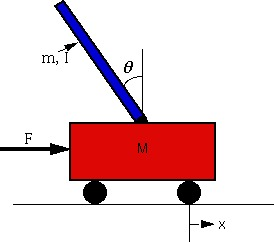
\includegraphics[width=0.5\linewidth]{invpen}
	\caption{Representação de um pêndulo invertido}
	\label{fig:invpen}
\end{figure}
Modelando esse sistema encontramos:
\begin{equation}
	\ddot{x} = \frac{\frac{F}{m} - gsin(\theta)cos(\theta) + l\dot{\theta}^2sin(\theta)}{\frac{M}{m} + sin(\theta)^2}
\end{equation}
\begin{equation}
	\ddot{\theta} = \frac{-\frac{Fcos(\theta)}{m} + \frac{(M+m)gsin(\theta)}{m} - l\dot{\theta}^2sin(\theta)cos(\theta)}{l(\frac{M}{m} + sin(\theta)^2)}
\end{equation}
Busca-se controlar a posição do carrinho $x$ enquanto mantendo a orientação vertical da haste. Esse sistema é altamente não linear a o equilíbrio $\theta = 0$ buscado é instável.

O sistema tratado tem os parâmetros:
\begin{equation}
	M = 0.455\ Kg
\end{equation}
\begin{equation}
	m = 0.21\ Kg
\end{equation}
\begin{equation}
	l = 0.61\ m
\end{equation}
\begin{equation}
	g = 9.8\ m/s^2
\end{equation}
\section{Dados para Treinamento}
Para os propósitos desse trabalho treinamos a rede neural utilizando uma combinação de controladores: consideramos dois problemas distintos, um que trabalha em torno do ponto de equilíbrio procurado e outro que leva nosso sistema para esse ponto de equilíbrio. 

Para as proximidades do ponto de equilíbrio foi utilizada uma combinação de controladores PD e um ganho de feedfoward no controle de posição do carrinho combinado com um controlador LQR que foca no controle do ângulo $\theta$. Essa estrutura de controle é a proposta nos demos do Matlab e apresenta um resultado bastante satisfatório.

Para levar o sistema ao ponto de equilíbrio um controlador bastante simples foi implementado: quando o sistema se encontra longe do ponto buscado $|\theta| > \frac{pi}{3}$ aplica-se uma força de intensidade constante e sinal idêntico à velocidade ângular $\dot{\theta}$ até que o pêndulo chegue a região de operação desejada.

Foi montada então a estrutura vista na figura \ref{fig:train} em que a saída de vários dos controladores foi saturada e simulamos esse sistema para uma referência de posição que muda aleatoriamente a cada 10 segundos e para condições iniciais de $\theta$ variando de $0$ a $2\pi$ com passos de $\frac{\pi}{18}$, cada uma dessas simulações tem uma duração de 50 segundos. Alguns dos resultados dessa simulações podem ser visto na figura \ref{fig:trainresults}

\begin{figure}[H]
	\centering
	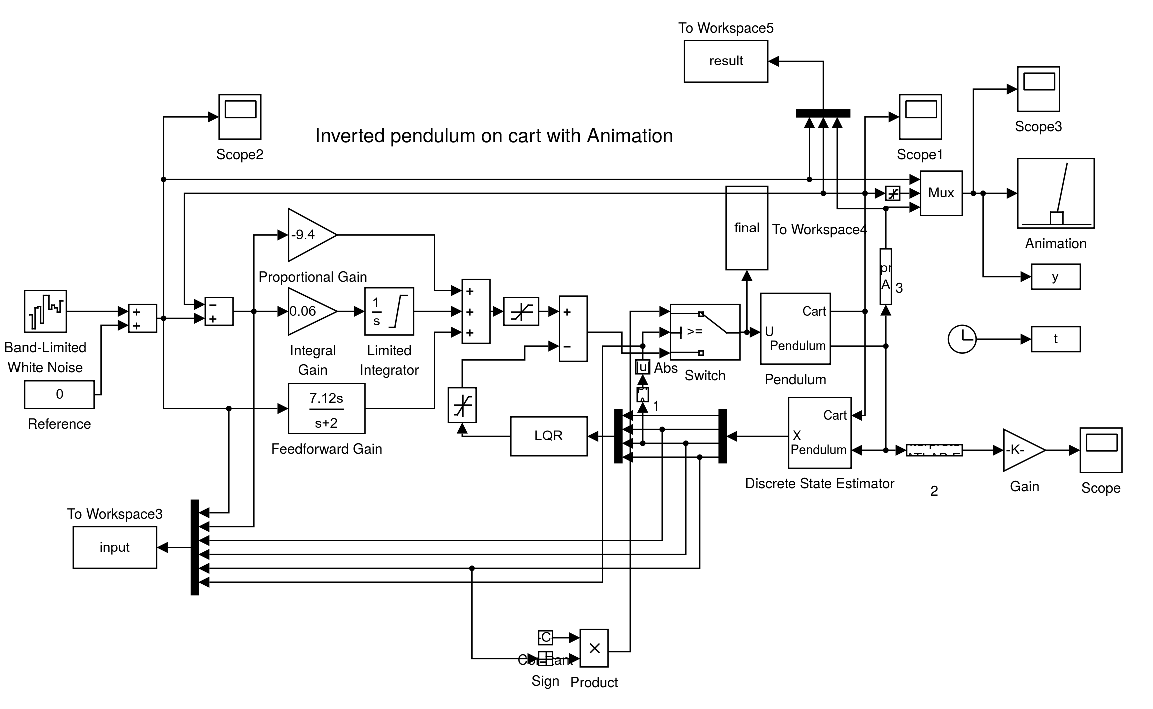
\includegraphics[width=0.7\linewidth]{train}
	\caption{Implementação Simulink do controlador para treinamento}
	\label{fig:train}
\end{figure}s are \quad and \qqua

%TODO Exportar e gerar subfigures
\begin{figure}[H]
	\centering
	\includegraphics[width=0.7\linewidth]{trainresults}
	\caption{Resultados da simulação de treinamento}
	\label{fig:trainresults}
\end{figure}


Exportamos como dados de entrada para o treinamento a referência e o erro em posição, a velocidade linear do carrinho, a velocidade e a posição angular do mesmo e o valor absoluto da posição angular normalizada para valores entre $-\pi$ e $\pi$. Esse último dado é utilizado como chave para a troca entre os controladores e por ser uma função complexa da posição angular escolhemos exportá-la afim de facilitar o treinamento da rede.
Como saída exportamos o sinal de controle: a força $F$ aplicada no carrinho.

Como nos primeiros treinamentos notamos que a rede estava tendo dificuldades para trabalhar com ângulos iniciais na faixa $\frac{pi}{2}$ à $\frac{3pi}{2}$ então aumentamos nossos dados de treinamento para incluir mais simulações saindo de condições iniciais nesse intervalo, com um passo de $\frac{\pi}{12}$ com uma duração de 20 segundos.

\section{A Rede}
Ou rede sustentabilidade é um partido político liderado por Marina Silva.

6 45 4 1
duas hidden layers
Treinado com Bayesian Regularization
https://www.mathworks.com/help/nnet/ug/improve-neural-network-generalization-and-avoid-overfitting.html
Umas 1000 epochs, erro de 0.7

\section{Resultados}
DEU BOM
\pagebreak

\end{document}

		
